%\documentclass[conference]{IEEEtran}
\documentclass[10pt,conference,anonymous]{IEEEtran}
\IEEEoverridecommandlockouts




\usepackage{inconsolata}
\usepackage{listings}

\lstset{language=Java,
basicstyle=\ttfamily\scriptsize,
%basicstyle=\ttfamily,
keywordstyle=\color{javapurple}\bfseries,
stringstyle=\color{pblue},
commentstyle=\color{javagreen},
morecomment=[s][\color{javadocblue}]{/**}{*/},
morecomment=[s][\color{gray}]{@}{\ },
numbers=left,
numberstyle=\tiny\color{black},
stepnumber=2,
numbersep=8pt,
tabsize=4,
showspaces=false,
showstringspaces=false,
breaklines=true,}

%%%%%%%%%%%%%%%%%%%%%%%%%%%%%%%%%%




\usepackage{adjustbox} % ajustar tabela ao tamanho da pagina

\usepackage{tikz}
\usetikzlibrary{matrix,fit,shapes,calc,positioning,shadows,arrows,shapes,backgrounds,decorations.markings,fadings}
\usepackage{graphicx}
\usepackage{multirow}
\usepackage[caption=false, font=footnotesize]{subfig}
\usepackage{wrapfig}
\usepackage{enumitem}
\usepackage{url}
%% helpers
\newcommand{\js}{JS}
\newcommand{\javascript}{JavaScript}
\newcommand{\es}{ES}
\newcommand{\ecmascript}{\es{}}
\newcommand{\tname}{TNAME}
\newcommand{\Comment}[1]{}
\newcommand{\numsubjects}{5}
\newcommand{\etal}{and colleagues'}
\newcommand{\ie}{i.e.}
\newcommand{\eg}{e.g.}
\newcommand{\cmark}{\ding{51}}%
\newcommand{\xmark}{{\color{red}\ding{55}}}%
\newcommand{\pGoodGood}{$\mathit{P}${\small\cmark\!\cmark}}%
\newcommand{\pGoodBad}{$\mathit{P}${\small\cmark\!\xmark}}%
\newcommand{\pBadDontCare}{$\mathit{P_?}$}%
\newcommand{\sfl}{SFL\xspace}
\newcommand{\ddg}{DDG\xspace}
\newcommand{\totfiles}{$\sim$38K}

%% annotations
\newif\ifdraftmode
%% Comment or uncomment the \draftmodetrue line.
\draftmodetrue
\ifdraftmode
 \newcommand{\Fix}[1]{\textbf{[[}{\color{red} #1}\textbf{]]}}
 \newcommand{\Mar}[1]{\textbf{[[Marcelo: }{\color{magenta} #1}\textbf{]]}}
 \newcommand{\Igor}[1]{\textbf{[[Igor: }{\color{blue} #1}\textbf{]]}}
 \newcommand{\note}[1]{\todo[inline,color=red!30,caption={}]{#1}}
\else
 \newcommand{\Fix}[1]{\relax}
 \newcommand{\Mar}[1]{\relax}
 \newcommand{\Igor}[1]{\relax}
 \newcommand{\note}[1]{\relax}
\fi

% For submitted version only.
\pagenumbering{arabic}

% Uncomment this if you need more space
%% \makeatletter
%% \def\@copyrightspace{\enlargethispage{-10pt}\relax}
%% \makeatother

\newcommand{\codesize}{\small}
\newcommand{\CodeIn}[1]{\mcodeid{#1}}
\newcommand{\CodeInM}[1]{\mcodeid{#1}}
% \|name| or \mathid{name} denotes identifiers and slots in formulas
\def\|#1|{\mathid{#1}}
\newcommand{\mathid}[1]{\ensuremath{\mathit{#1}}}
% \<name> or \codeid{name} denotes computer code identifiers
\def\<#1>{\codeid{#1}}
\newcommand{\codeid}[1]{\ifmmode{\mbox{\codesize\ttfamily{#1}}}\else{\codesize\ttfamily #1}\fi}
\def\<#1>{\mcodeid{#1}}
\newcommand{\mcodeid}[1]{\mbox{\codesize\ttfamily{#1}}}

%% thumbs up down
\newcommand*{\RightThumbsUpAux}[1]{%
  \begingroup
    \sbox0{Ag}%
    \raisebox{-\dp0}{%
      \includegraphics[{%
        height=\dimexpr\dp0+\ht0\relax,
        #1%
      }]{thumbsup.pdf}%
    }%
  \endgroup
}
\newcommand*{\RightThumbsUp}{%
  \RightThumbsUpAux{}%
}
\newcommand*{\RightThumbsDown}{%
  \RightThumbsUpAux{origin=c,angle=180}%
}
\newcommand*{\LeftThumbsUp}{%
  \scalebox{-1}[1]{\RightThumbsUp}%
}
\newcommand*{\LeftThumbsDown}{%
  \scalebox{-1}[1]{\RightThumbsDown}%
}

\newcommand{\checkm}{Y}
\newcommand{\crossmark}{N}
%\begin{wraptable}[20]{t}[0pt]{0.5\textwidth}

\newcommand{\totalTestFiles}{38,369}
\newcommand{\totalTestFilesCompileInAll}{35,939}
\newcommand{\totalTestFilesPassInAll}{24,493}
\newcommand{\nofuzzAll}{209}
\newcommand{\nofuzzBugs}{\Fix{XX}}
\newcommand{\nofuzzDuplicates}{63}
\newcommand{\nofuzzFalsePositives}{24}
\newcommand{\nofuzzHITotal}{177}
\newcommand{\nofuzzLOTotal}{32}
\newcommand{\nofuzzTotalFiles}{977} % conflicting files
\newcommand{\nofuzzFilesHI}{940} % conflicting files HI
\newcommand{\nofuzzFilesLO}{37} % conflicting files LO

\newcommand{\nofuzzBucketsBugsHI}{\Fix{124}} % buckets reported (including dups)
\newcommand{\nofuzzBucketsBugsLO}{\Fix{11}} % buckets reported
\newcommand{\nofuzzDupsHI}{\Fix{X}}
\newcommand{\nofuzzDupsLO}{\Fix{Y}}

% continue updating bugs table
\newcommand{\tableBugsNum}{\Fix{26}}

%% anonymize

\newcommand{\anonym}[1]{{\tiny\colorbox{black}{#1}}}

%% names
\newcommand{\radamsa}{radamsa}
\newcommand{\quickfuzz}{quickfuzz}

\newcommand{\jsc}{JavaScriptCore}
\newcommand{\veight}{V8}
\newcommand{\chakra}{Chakra}
\newcommand{\smonkey}{SpiderMonkey}
\newcommand{\jerry}{JerryScript}

\newcommand{\lo}{lo}
\newcommand{\hi}{hi}


\begin{document}

\title{Finding Bugs in JavaScript Engines with Differential
  Testing---an Experience Report}

%% \author{
%% \IEEEauthorblockN{Sabrina Souto}
%% \IEEEauthorblockA{State University of Para\'iba\\
%% Para\'iba, Brazil\\
%% sabrinadfs@gmail.com}
%% \and
%% \IEEEauthorblockN{Marcelo d'Amorim}
%% \IEEEauthorblockA{Federal University of Pernambuco\\
%%   Pernambuco, Brazil\\
%%   damorim@cin.ufpe.br}
%% \and
%% \IEEEauthorblockN{Rohit Gheyi}
%% \IEEEauthorblockA{Federal University of Campina Grande\\
%%   Para\'iba, Brazil\\
%%   rohit@dsc.ufcg.edu.br}
%% }

\maketitle

\begin{abstract}
\end{abstract}

\begin{IEEEkeywords}
...
\end{IEEEkeywords}

\section{Introduction}

JavaScript (\js{}) is one of the most popular programming languages of
today~\cite{business-insider,stackify}. The \js{} specification
changes relatively frequently to accommodate the pressing demands of
the community. For example, the JS specification went through a severe
change recently called by the name of ECMAScript6
(ES6)~\cite{es6-features}.  These changes often entail sensible
changes in engine implementations~\cite{kangax} that could lead to
errors, including regressions. Automated techniques can help finding
bugs, but the lack of executable specifications limits their ability
to detect errors not manifested by universal oracles.

This paper reports on a study to find those kinds of bugs in
JavaScript engines. The goal of the study is to improve quality of
existing \js{} engines by improving the bug finding process. We used
differential testing~\cite{Brumley-etal-ss07}, a technique that has
been applied in a variety of
contexts~\cite{Yang-etal-pldi11,Chen-etal-fse2015,Argyros-etla-ccs16,Chen-etal-pldi16,petsios-etal-sp2017,SivakornAPKJ17}
to address the oracle problem. Differential testing leverages the
diversity across system's implementations to detect anomalous
behavior. \Mar{this needs work$\rightarrow$}
\Fix{but it has not been thoroughly explored to find functional bugs in JS
engines. The closest work was done by Patra and
Pradel~\cite{patra2016learning}, where they evaluated their proposed
language-agnostic fuzzer to find cross-browser HTML+JS
discrepancies. This project aims at building and evaluating an
infrastructure for differential testing of runtime engines, such as
the JS engine or WebAssembly's. The sensible parts of the
infrastructure are the checks of input validity (as to reduce
waste/cost) and output correctness (as to reduce false positives).}

\section{Infrastructure}
\label{sec:design}


%\begin{wrapfigure}[10]{r}[0pt]{0.45\textwidth}
\begin{figure}[h]
  \centering
  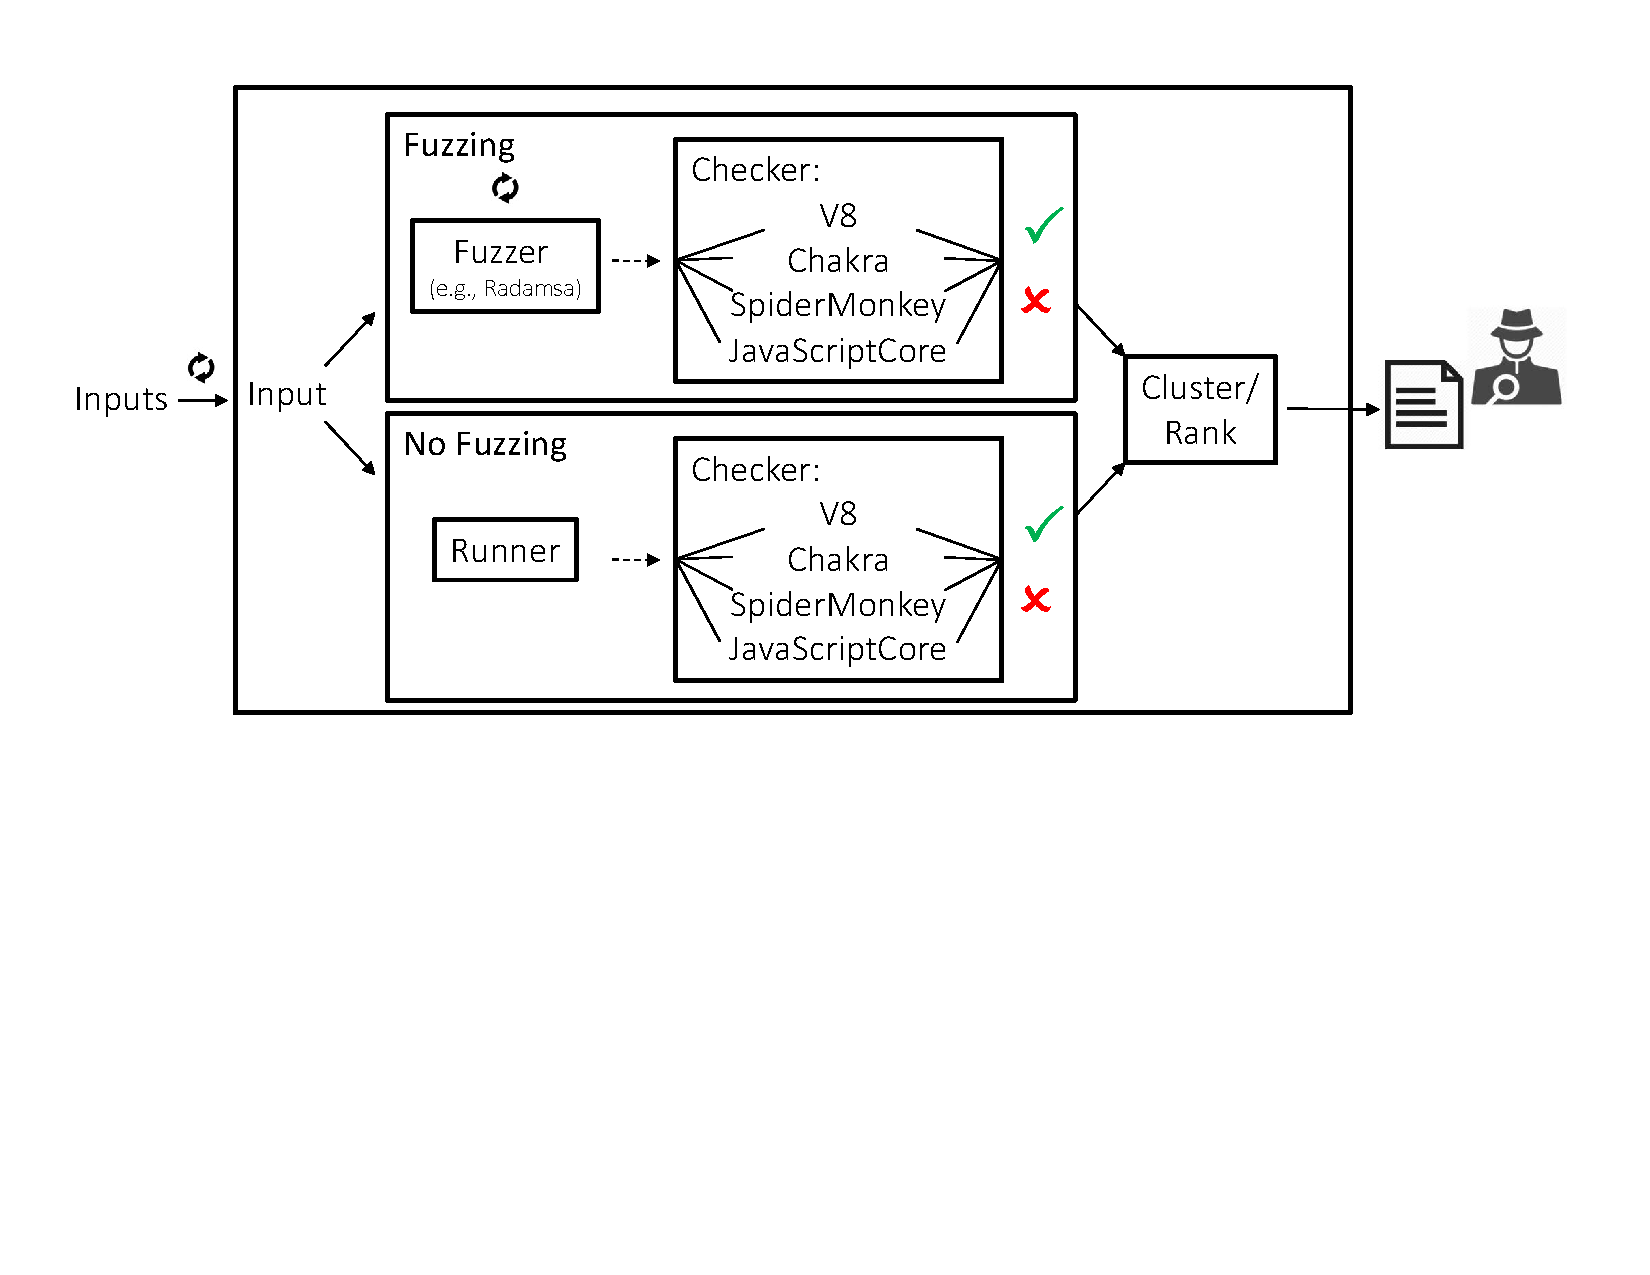
\includegraphics[trim=20 350 200 0,clip,width=0.45\textwidth]{google-awards-workflow}
  \caption{\label{fig:workflow}Infrastructure.}
\end{figure}

Figure~\ref{fig:workflow} illustrates the workflow of the
infrastructure we used in this study. Arrowed lines indicate control
flow (dashed) and data flow (filled); lines with no arrow denote
encapsulation. The bug-finding process takes on input JS files
originating from the regression test suites of various JS engines. It
is worth noting that we found online regression suites for a total of
\Fix{YY} JS engines.\Mar{show table with name and count of JS files}
If input fuzzing~\cite{fuzz-testing-history} is not selected, the
oracle checks whether or not the output is consistent across all
engine implementations. In case the test passes in all engines or
fails in all engines (\ie{}, the output is consistent), the
infrastructure discards the corresponding input. Otherwise, it
considers the input as potentially fault-revealing; hence interesting
for human inspection. If fuzzing is selected, new inputs are obtained
from a given input using some off-the-shelf fuzzer; the workflow is
similar to that of no fuzzing. Several fuzzing methods have been
proposed in the past, varying with respect to how new inputs are
generated (\eg{}, coverage-based~\cite{afl,honggfuzz},
grammar-based~\cite{grammarinator,jsfunfuzz}, and
random-based~\cite{radamsa}). \Mar{which ones we covered? why is this
  relevant?}

The infrastructure outputs a list of warnings for human inspection.
To reduce the number of false alarms, we clustered warnings in two
groups, reflecting their likelihood to manifest a real bug. The HI
group includes those inputs that manifest anomaly directly by the test
(or its close neighborhood) as opposed to anomaly in some JS
function. The rationale is that the test was able to execute to
completion without violating any internal checks of the API, but
failed to satisfy some check of the test. The LO group, in contrast,
includes those cases where the anomaly was observed executing some JS
function. We found that engine implementations often check
pre-conditions of API functions differently, leading to premature
failures. Most of the inputs in this category failed to satisfy the
pre-condition check of some, but not all engines. Although we did find
real bugs from warnings manifested in this category, the proportion is
much lower compared to the HI category--only 12\% of the reals bugs we
found originated from the LO category.\Mar{can we detect dups mining
  issue trackers?}

\Mar{show real examples of HI and LO and provide the
  rationale for such classification.}

%% selects randomly one of the inputs to fuzz with a
%% given tool, say the black-box fuzzer Radamsa~\cite{radamsa}. Each fuzzing iteration produces a new
%% file. For grammar-agnostic fuzzers, like Radamsa, the infrastructure
%% can discard syntactically invalid inputs using an external parser for
%% the input language; semantically invalid inputs can be prevented with
%% with linters. Once the input is found to be likely valid, the
%% infrastructure invokes the oracle to check correctness. 


% \section{Related Work}
% Differential testing with fuzzing can improve the quality of programs
% Yang et al. \cite{yang-2011-finding}

%% \Mar{rule of thumb: explain the
%%   contribution/novelty, then results achieved, and then how it relates
%% with our proposal.}
%% \Mar{this is not clear$\rightarrow$}Yang et al. \cite{yang-2011-finding} proposed CSmith\footnote{\url{http://embed.cs.utah.edu/csmith/}}, a grammar-fuzzer 
%% of C programs to generate invalid entries\Fix{the goal of a
%%    fuzzer is to generate valid inputs/entries. this is strange}\MAB{the
%%   goal is to generate valid programs without undefined behavior to
%%   facilitate differential testing} and
%% find bugs in several C compilers\Fix{it is strange that you don't mention differential
%%   testing, which is central in CSmith, and the use of LLVM and GCC as
%%   oracles.}.\Mar{this is just listing fuzzers. don't do this. try to
%%   follow rule of thumb above.}Similar fuzzers involving grammar and rules are found in Holler et al. \cite{holler-2012-fuzzing} 
%% that exposes the LangFuzz to generate entries based in code fragments 
%% (language grammar, sample code, test suite) and the tool Mozilla 
%% Funfuzz\footnote{\url{https://github.com/MozillaSecurity/funfuzz}}
%% that implements a fuzzer based on JavaScript language to improve the 
%% testing for SpiderMonkey engine, the interpreter of Mozilla Firefox.
%% \Fix{...}

\section{Current Results}
\label{sec:results}

\newcommand{\checkm}{Y}
\newcommand{\crossmark}{N}
%\begin{wraptable}[20]{t}[0pt]{0.5\textwidth}

\begin{table*}
  \vspace{-3ex}
%  \scriptsize
  \centering
  \caption{List of bug reports issued by our team from April 12 to May
    24, 2018.}
  \label{tab:bugs}
  \begin{tabular}{cccccc}
    \toprule
    Issue\#    & Date & Fuzz & Engine  & Status  & \multicolumn{1}{c}{Url}   \\
    \midrule    
    1  & 4/12 & \checkm & Chakra   & \textbf{Fixed}  & \href{https://github.com/Microsoft/ChakraCore/issues/4978}{\#4978}      \\ 
    2  & 4/12 & \checkm & Chakra   & Rejected  & \href{https://github.com/Microsoft/ChakraCore/issues/4979}{\#4979}      \\
    3  & 4/14 & \checkm & JavascriptCore  & New & \href{https://bugs.webkit.org/show\_bug.cgi?id=184629}{\#184629}        \\
    4  & 4/18 & \crossmark & JavascriptCore  & New  & \href{https://bugs.webkit.org/show\_bug.cgi?id=184749}{\#184749}        \\
    5  & 4/23 & \crossmark & Chakra  & \textbf{Confirmed}  & \href{https://github.com/Microsoft/ChakraCore/issues/5033}{\#5033}       \\
    6  & 4/25 & \checkm & Chakra  & \textbf{Fixed}     & \href{https://github.com/Microsoft/ChakraCore/issues/5038}{\#5038}      \\
    7  & 4/29 & \crossmark & Chakra  & \textbf{Confirmed}   &
    \href{https://github.com/Microsoft/ChakraCore/issues/5065}{\#5065}
    \\
    \midrule
    \multirow{2}{*}{8}  & \multirow{2}{*}{4/29} &  \multirow{2}{*}{\crossmark} & Chakra & \textbf{Confirmed} &    \href{https://github.com/Microsoft/ChakraCore/issues/5067}{\#5067} \\
                        &  &                       &
    JavascriptCore & New &    \href{https://bugs.webkit.org/show\_bug.cgi?id=185130}{\#185130}    \\
    \midrule    
    9  & 4/29 & \checkm & JavascriptCore  & New  &    \href{https://bugs.webkit.org/show\_bug.cgi?id=185127}{\#185127}    \\
    \midrule    
    \multirow{2}{*}{10} & \multirow{2}{*}{4/30}  & \multirow{2}{*}{\checkm} & Chakra & \textbf{Confirmed} &    \href{https://github.com/Microsoft/ChakraCore/issues/5076}{\#5076} \\    
                        &                        &        &
    JavascriptCore & New &
    \href{https://bugs.webkit.org/show\_bug.cgi?id=185156}{\#185156}
    \\
    \midrule    
    11 & 5/02 & \checkm & JavascriptCore  & New & \href{https://bugs.webkit.org/show\_bug.cgi?id=185197}{\#185197}\\
    12 & 5/02 & \crossmark & JavascriptCore & New  & \href{https://bugs.webkit.org/show\_bug.cgi?id=185208}{\#185208}\\
    13 & 5/10 & \checkm & Chakra & \textbf{Confirmed} & \href{https://github.com/Microsoft/ChakraCore/issues/5128}{\#5128} \\
    14 & 5/17 & \checkm & Chakra & \textbf{Confirmed} & \href{https://github.com/Microsoft/ChakraCore/issues/5182}{\#5182} \\
    15 & 5/17 & \crossmark & Chakra & \textbf{Confirmed} & \href{https://github.com/Microsoft/ChakraCore/issues/5187}{\#5187} \\
    16 & 5/21 & \crossmark & Chakra & \textbf{Confirmed} & \href{https://github.com/Microsoft/ChakraCore/issues/5203}{\#5203} \\
    17 & 5/24 & \checkm & JavascriptCore & New  & \href{https://bugs.webkit.org/show\_bug.cgi?id=185943}{\#185943}\\
   \bottomrule     
  \end{tabular}
\end{table*}

%% Although there are many features yet to implement in our
%% infrastructure, 

The workflow described in Section~\ref{sec:design} is currently
functional. This section shows preliminary results obtained with our
infrastructure providing some evidence that finding bugs in JS runtime
engines with differential testing is promising. Table~\ref{tab:bugs} shows the list of bugs we
reported on issue trackers of different engines in the period of 42 days. For example, bug \# 6 was manifested by the JS code \CodeIn{var
  a = \{valueOf:~function()\{return ``\textbackslash{}x00''\}\}
  assert(+a === 0)\}}.  The object property \CodeIn{valueOf} stores a
function that returns a primitive value identifying the target
object~\cite{valueof}. That function returns an empty string in the
original version of this code. The modified version of the code
returns a string representation of a null character (called
\CodeIn{NUL} in ascii). The unary plus expression ``\CodeIn{+a}", appearing in the assertion,
is equivalent to the abstract operation \CodeIn{ToNumber(a.valueOf())}
that converts a string to a number, otherwise the operation returns NaN 
(Not a Number)\cite{unary-plus}. For this case, Chakra evaluates the unary
plus to NaN as expected, as the null character cannot be converted. As result, the test fails as
expected. Chakra, in contrast, incorrectly converts the string to zero, making the test to pass.

So far, ten of the bugs we reported
were confirmed, two of which were fixed. One bug report we
submitted was rejected on the basis that the offending JS file
manifested an expected incompatibility across engine
implementations.
Note from the table that all bug
reports still waiting for confirmation are associated with the
JavaScriptCore engine (JSC). A closer look at the JSC issue tracker
showed that the triage process is very slow for that engine. As of
now, we did not find any new bug on SpiderMonkey and V8; the bugs we
found were duplicates and were not reported. Finally, it is
worth noting that 7 of the 17 JS files that manifested
discrepancies were \emph{not} produced with fuzzing (column
``Fuzz''). These are test files from suites of different engines. This
observation emphasizes the importance of continuously collecting test suites from
multiple sources; today, we use test suites from seven different open
source engines, including a total of 30K test files.

%\section*{Acknowledgment}

%\bibliographystyle{IEEEtran}
\bibliographystyle{plain}
\bibliography{references,../docs/google-research-awards-latam/tmp}

\end{document}
